\section{Оптические инструменты. Микроскоп. Телескоп (труба Кеплера, труба Галилея). Угловое увеличение телескопа.}

\subsection{Микроскоп}

\begin{figure}[H]
	\centering
	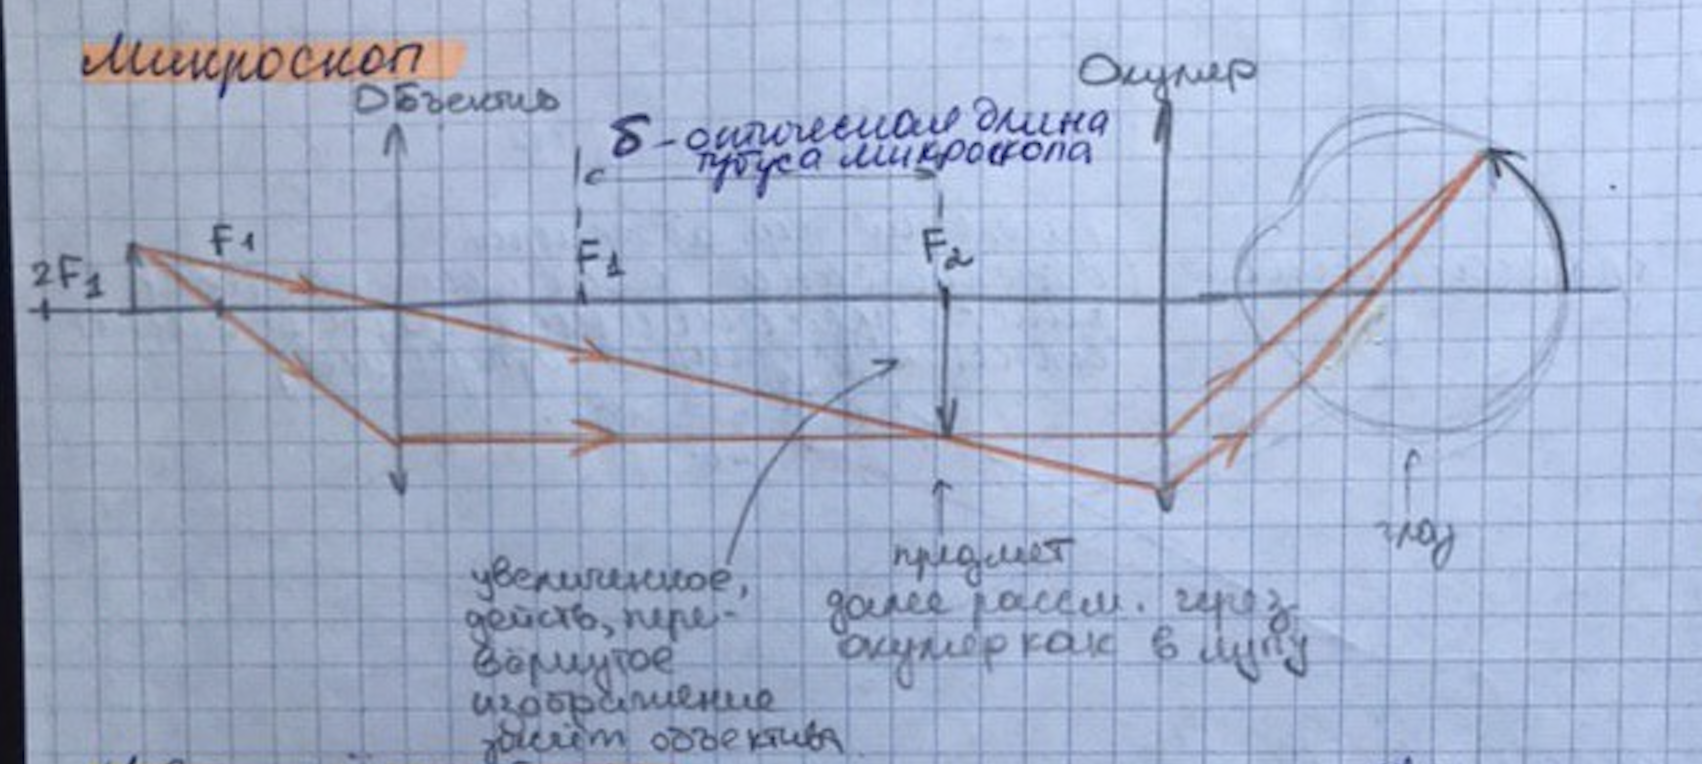
\includegraphics[width=\textwidth]{6_3}
	\caption{Микроскоп. Извините, я усталь.}
\end{figure}

\subsection{Труба Кеплера}

\begin{figure}[H]
	\centering
	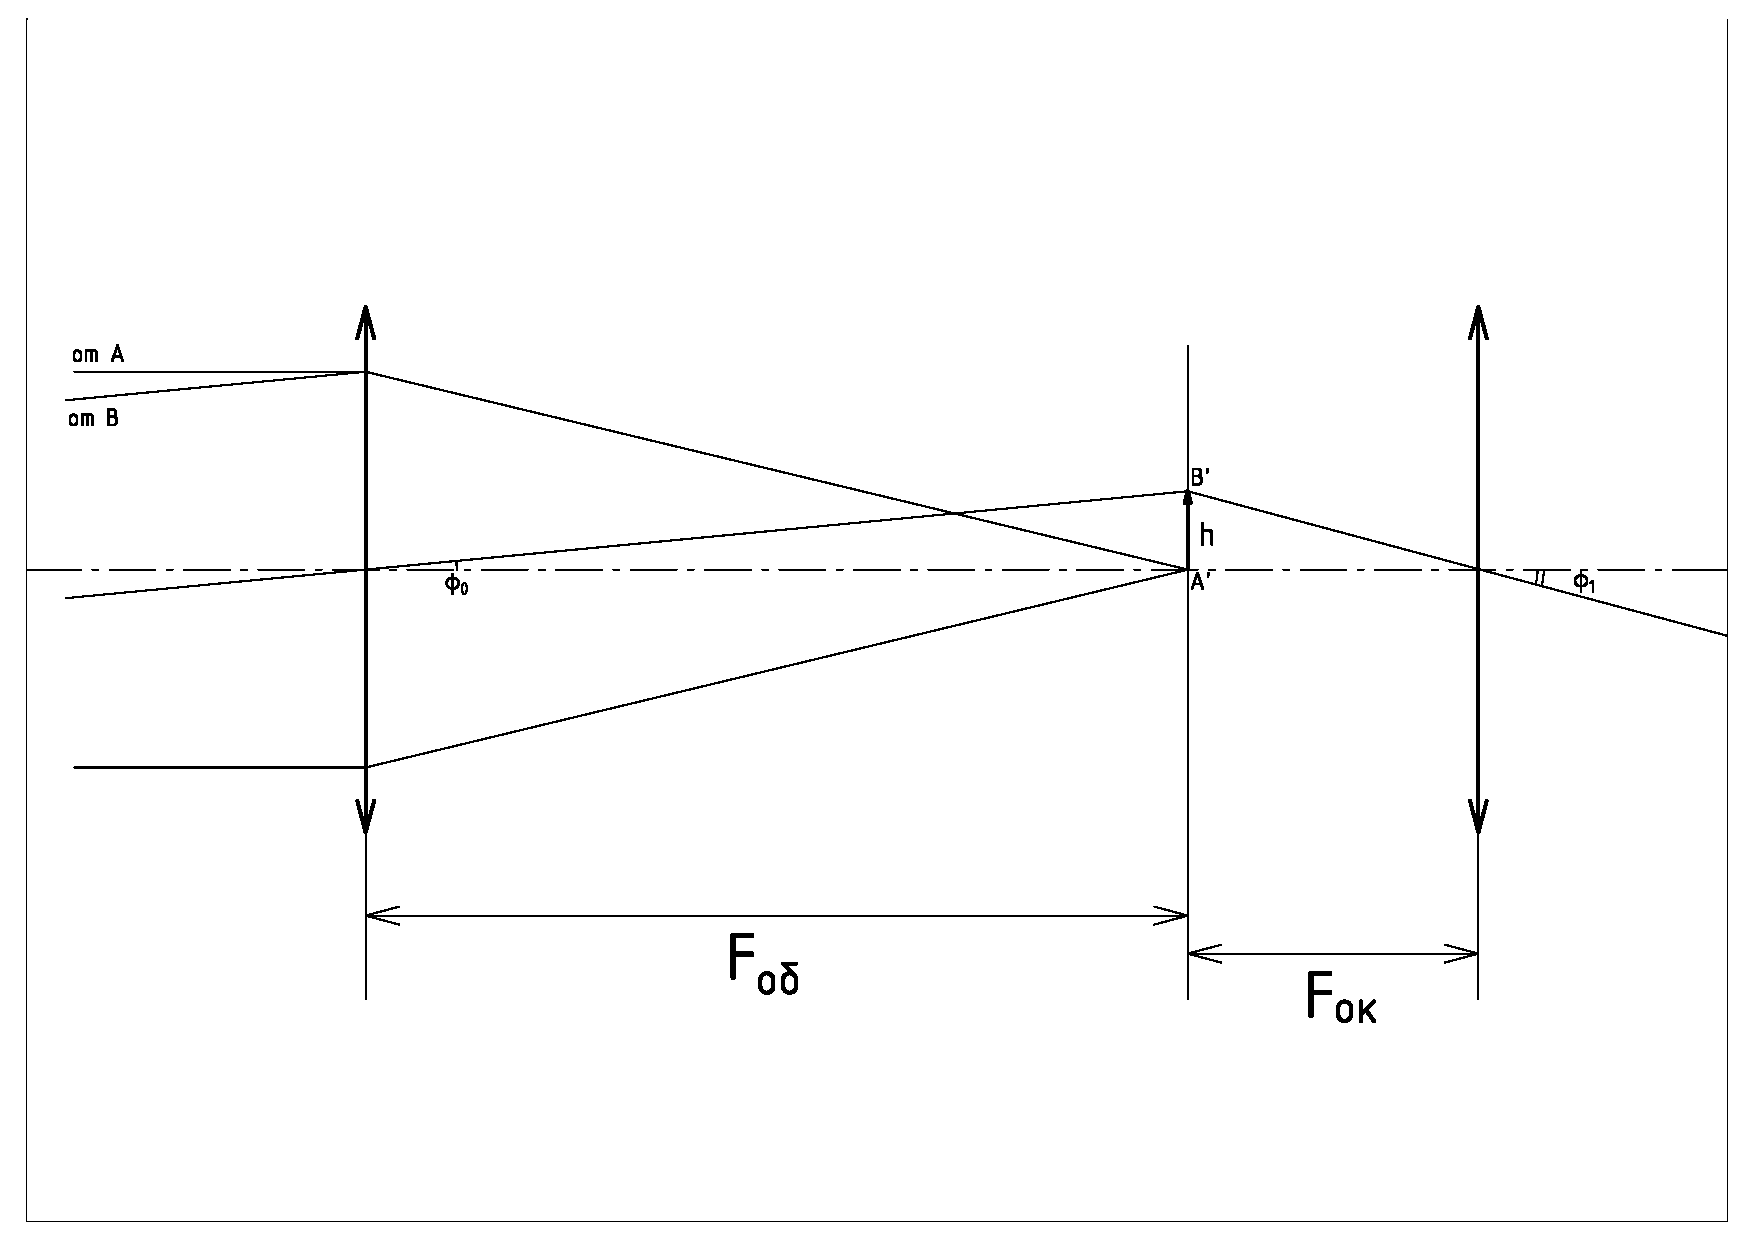
\includegraphics[width=\textwidth]{6_1}
	\caption{Труба Кеплера}
\end{figure}

Из подобия мы сразу можем заявить:

\begin{equation*}
	\frac{D_{\text{об}}}{F_{\text{об}}} = \frac{D_{\text{ок}}}{F_{\text{ок}}}
\end{equation*}

Где $D$ --- диаметр.

Пусть мы наводимся на далекий объект (луну, например). Рассмотрим два пучка от точки $A$ и $B$ соответственно. При прохождении через первую линзу они дадут изображение $A'B'$ в фокальной плоскости, пусть его высота $h$. Затем луч от точки $B$ выйдет из второй линзы (окуляра) под углом $\phi_1$. Введем \textbf{угловое увеличение телескопа} $\gamma$:

\begin{equation*}
	\gamma = \frac{\tg \phi_1}{\tg\phi_0} = \frac{h / F_{\text{ок}}}{ h / F_{\text{об}}} = \frac{F_{\text{об}}}{F_{\text{ок}}} = \frac{D_{\text{об}}}{D_{\text{ок}}}
\end{equation*}

\subsection{Труба Галилея}

В случае трубы Галилея ситуация ровно такая же, как в случае трубы Кеплера, однако линза окуляра рассеивающая, а не собирающая. Из-за этого фокус объектива должен совпасть с \textbf{задним} фокусом окуляра (см. рисунок). Больше от этого ничего не меняется.

\begin{figure}[H]
	\centering
	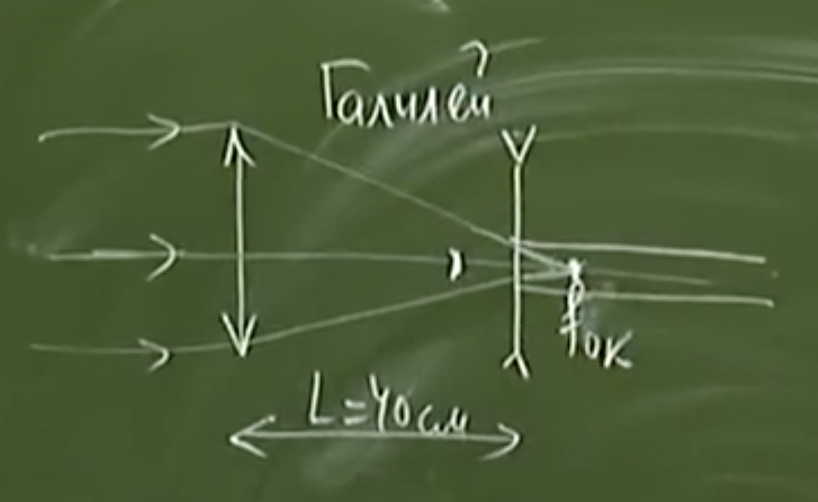
\includegraphics[width=\textwidth]{6_2}
	\caption{Труба Галилея}
\end{figure}
